
\section{Johtajarusakot}

\textit{Monipuolisen partiotoiminnan mahdollistavat aktiiviset johtajat. Myös
kaikille heille partio on harrastus. Moni viihtyy partiossa ekaluokkalaisesta
\mbox{aikuiseksi} asti, sillä kaiken ikäisille riittää uutta koettavaa. Tässä Tassun
juttusarjassa tutustumme tarkemmin KuRu:n johtajiin.}

\vspace*{0.32cm}
% \noindent Tällä kertaa mennään ajassa 20 vuotta taaksepäin, ja katsotaan mitä
% \mbox{KuRu:n} kolkat puuhasivat heidän syysretkellään vuonna 2004:

\newtcolorbox{FaktaLaatikko}[1][]{%
    enhanced,
    before skip=2mm,after skip=2mm, 
    width=\textwidth, boxrule=0.2mm, % width of the sticky note
    colback=white, colframe=kuru, % Colors
    attach boxed title to top right={xshift=0cm,yshift*=0mm-\tcboxedtitleheight},
    varwidth boxed title*=-3cm,
    % The titlebox:
    boxed title style={frame code={%
        \path[left color=kuru,right color=kuru,
        middle color=kuru]
        ([xshift=-0mm]frame.north west) -- ([xshift=0mm]frame.north east)
        [rounded corners=0mm]-- ([xshift=0mm,yshift=0mm]frame.north east)
        -- (frame.south east) -- (frame.south west)
        -- ([xshift=0mm,yshift=0mm]frame.north west)
        [sharp corners]-- cycle;
        },interior engine=empty,
    },
    sharp corners,rounded corners=southeast,arc is angular,arc=3mm,
    % The "folded paper" in the bottom right corner:
    underlay={%
        \path[fill=kuru!80!black] ([yshift=3mm]interior.south east)--++(-0.4,-0.1)--++(0.1,-0.2);
        \path[draw=kuru,shorten <=-0.05mm,shorten >=-0.05mm,color=kuru] ([yshift=3mm]interior.south east)--++(-0.4,-0.1)--++(0.1,-0.2);
        },
    % drop fuzzy shadow, % Shadow
    % fonttitle=\bfseries, 
    title={#1}
}

\noindent \textbf{\Large Esittelyssä Leo}

\begin{multicols}{2}

\subsection*{Partiossa}
Tänä vuonna tulee täyteen 10 vuotta partiossa! Aloitin tosiaan partion pienenä ekaluokkalaisena vuonna 2015.

\vspace*{0.16cm}
\noindent\textbf{Millaisia partiotehtäviä sinulla on juuri nyt?}\\
Tällä hetkellä johdan seikkailijavartiota ja toimin (ainakin nimellisesti) lippukunnan varainhankintavastaavana.

\vspace*{\fill}
\columnbreak
\subsection*{``Siviilissä''}
Siviilissä opiskelen lukiossa toista vuotta ja kesäisin satunnaisia töitä. Nyt pari kesää ollut leiriohjaajana!

\vspace*{0.16cm}
\noindent\textbf{Mitä muuta harrastat?}\\
Partion lisäks harrastan fiiliksestä riippuen kaikkea sekalaista taiteilua ja muuta sekoilua. Soitan bändissä kitaraa ja laulan, jonka lisäks teen kuvataidetta ja käsitöitä aina kun huvittaa. Tällä hetkellä oon innostunut geokätköilystä!

\end{multicols}

% \vspace*{0.32cm}
% \vspace*{-0.64cm}
\begin{FaktaLaatikko}[Leo]

\begin{multicols}{2}
\vspace*{-0.64cm}
\vspace*{-0.16cm}
\begin{itemize}
\item Oon 17-vuotias ja asun Vantaan Hiekkaharjussa
\item \textbf{Kuuntelen mieluiten:} Kuuntelen paljon kaikkea erilaista musaa, mut tällä hetkellä kuuntelen paljon folkia ja rockia
\item \textbf{Katson mieluiten:} Oon tosi huono kattomaan yhtään mitään mut mun lempisarja on ehdottomasti Criminal Minds!
\item \textbf{Lautasella mieluiten:} jotain kotitekosta, mausteista kasvisruokaa!
\end{itemize}
\columnbreak

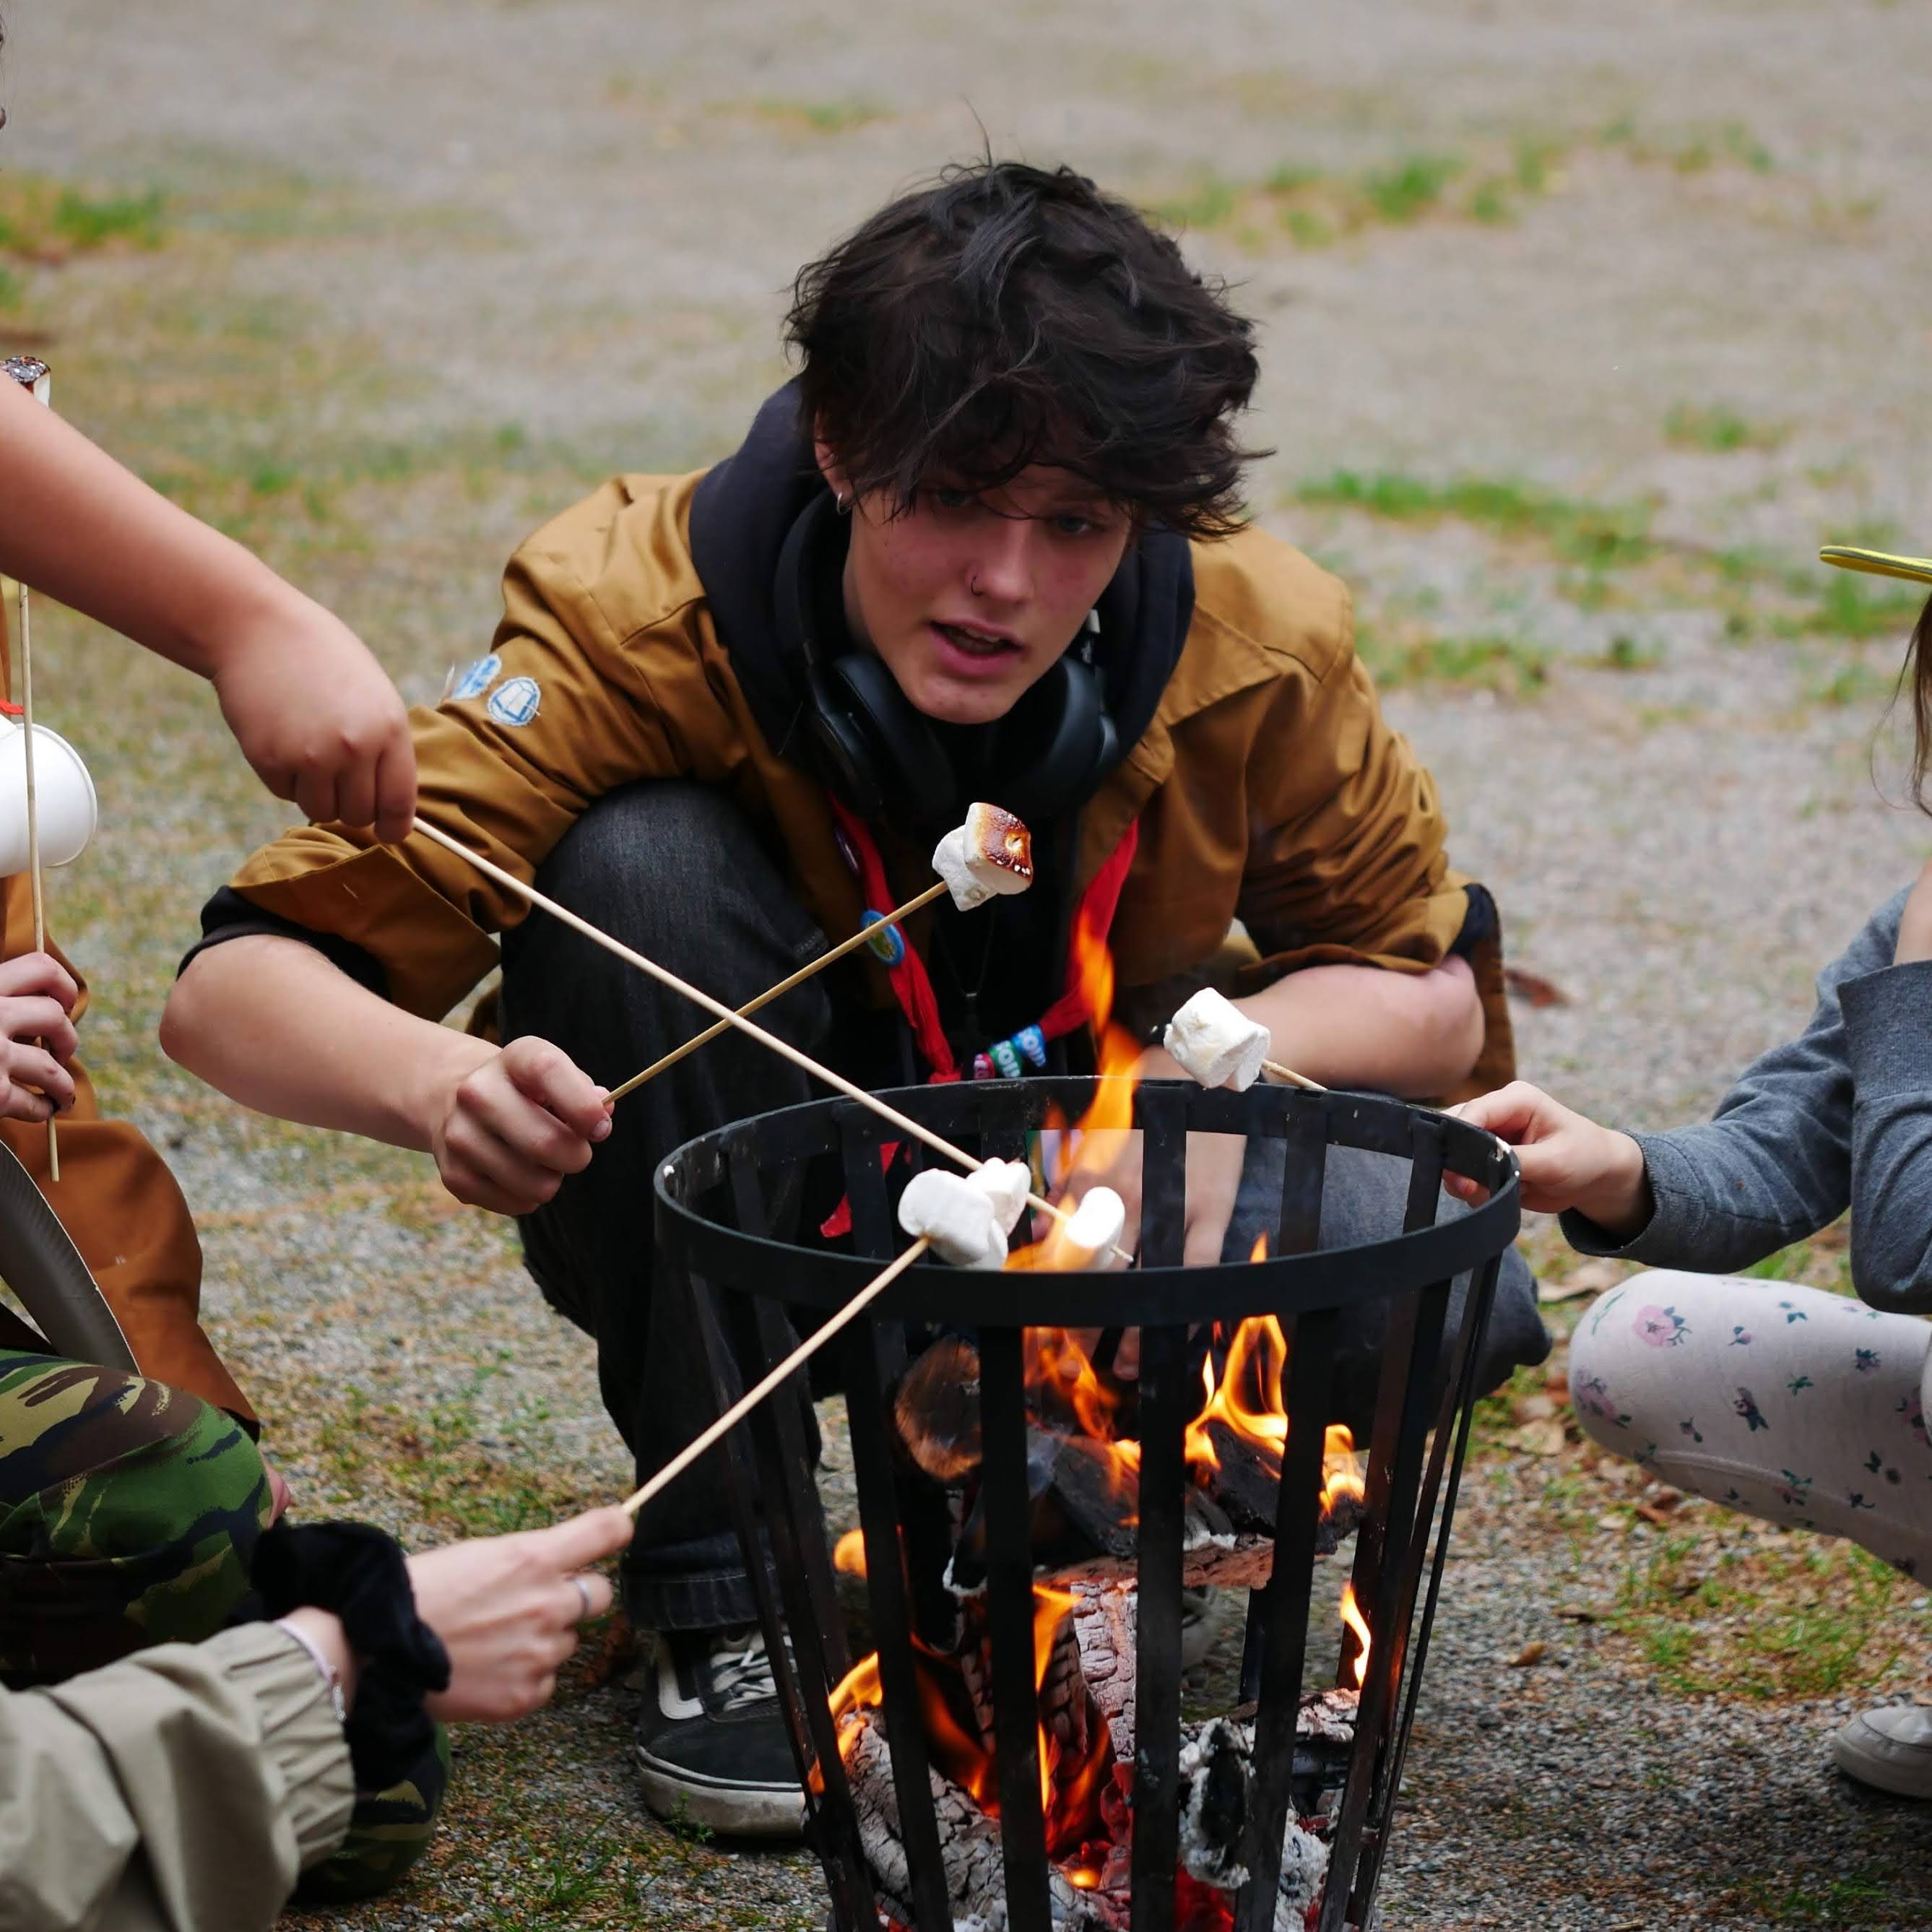
\includegraphics[width=1.02\columnwidth]{assets/johtajarusakot-leo.jpg}
\end{multicols}

\end{FaktaLaatikko}
\vspace*{-0.64cm}
